% Generated by scripts/plot_association_cases.py from audited JSON.
\subsection{Audited examples of changed decisions}

In the held-out CyBench challenge \texttt{back\_to\_the\_past}, a Human trace with 48 extracted commands and an Agent trace with 47 commands share the task label but have command-cosine similarity 0.215. The behavior ranker rejects the pair ($0.5088 < 0.5131$); the mode-aware ranker accepts it ($0.5482 \geq 0.5127$). The mode detector's raw Agent scores are 0.3683 and 0.7221, respectively. This pair illustrates how predicted mode information can change a borderline matching decision.

The same representation also introduces a cross-challenge link: a Human \texttt{back\_to\_the\_past} trace and an Agent \texttt{glacier-exchange} trace change from rejection ($0.4738 < 0.5131$) to acceptance ($0.5161 \geq 0.5127$). Figure~\ref{fig:association-cases} locates both the value and the design challenge: execution-mode context can recover cross-mode matches, while distinguishing the underlying task remains essential to controlling spurious links. Case selection and full trace identifiers are documented in the appendix.

\begin{figure}[t]
\centering
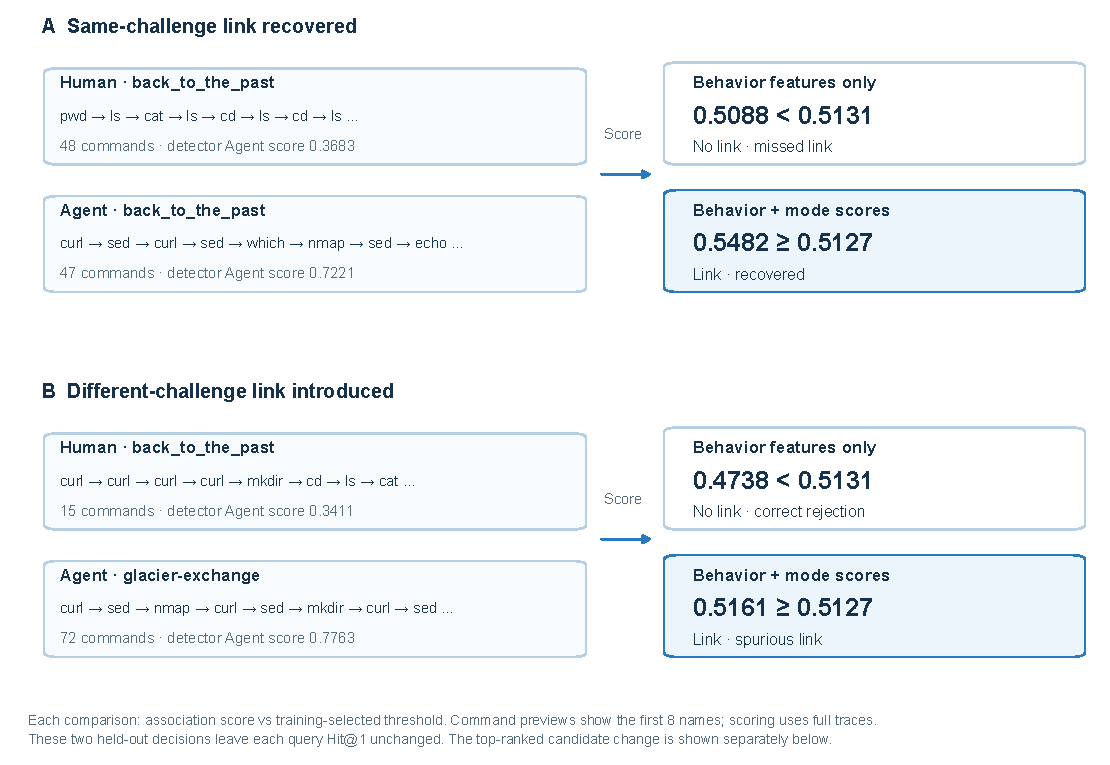
\includegraphics[width=\linewidth]{association_cases_v1.pdf}
\caption{Audited Human--Agent pairs from held-out CTF tasks. Each numeric comparison shows an association score against its training-selected threshold. The common 20\% training false-merge target permits method-specific thresholds. Only command-name previews are displayed; scoring uses complete normalized trajectories. Source labels are shown for interpretation, while the ranker uses predicted mode scores. These examples explain a recovered same-challenge link and a new cross-challenge error.}
\label{fig:association-cases}
\end{figure}
